\documentclass[a4paper]{article}

\usepackage{graphicx}
\usepackage{float}
\usepackage{listings}
\usepackage{xcolor}
\usepackage{graphicx}

\definecolor{codegreen}{rgb}{0,0.6,0}
\definecolor{codegray}{rgb}{0.5,0.5,0.5}
\definecolor{codepurple}{rgb}{0.58,0,0.82}
\definecolor{backcolour}{rgb}{0.95,0.95,0.92}

\lstdefinestyle{mystyle}{
    backgroundcolor=\color{backcolour},   
    commentstyle=\color{codegreen},
    keywordstyle=\color{magenta},
    numberstyle=\tiny\color{codegray},
    stringstyle=\color{codepurple},
    basicstyle=\ttfamily\footnotesize,
    breakatwhitespace=false,         
    breaklines=true,    captionpos=b,                    
    keepspaces=true, numbers=left,                    
    numbersep=5pt, showspaces=false,                
    showstringspaces=false, showtabs=false, tabsize=2}
\lstset{style=mystyle}

\usepackage[utf8x]{inputenc}
\usepackage{fancyhdr}
\usepackage{lastpage}
% For figures and stuff
\usepackage{graphicx, wrapfig, subcaption, setspace, booktabs}
\usepackage[T1]{fontenc}
% Change for different font sizes and families
\usepackage[font=small, labelfont=bf]{caption}
\usepackage{fourier}
\usepackage[]{microtype}


\newcommand{\HRule}[1]{\rule{\linewidth}{#1}}
\onehalfspacing
\setcounter{tocdepth}{5}
\setcounter{secnumdepth}{5}

\usepackage[a4paper,top=2.5cm,bottom=2cm,left=2.5cm,right=2.5cm,marginparwidth=1.8cm]{geometry}
\pagestyle{fancy}


\setlength\headheight{15pt}
\fancyhead[L]{} 
\fancyhead[R]{Group 21}

\linespread{1.4}

%-----------------------------------------BEGIN DOC----------------------------------------
\begin{document}
\title{{\Huge \textbf{Bank Run: The downfall of First Republic Bank}{\large\linebreak\\}}{\Large \textit{In-depth analysis of the collapse of First Republic Bank and its comparison with Silicon Valley Bank using the Diamond-Dybvig model}\linebreak\linebreak}}

\author{Hanshuo Ma
\\ \\ \\
\textbf{University of Toronto at Mississauga} \\
Department of Economics \\ \\
Professor Yingnan Zhao \\
ECO349H5 S - Money, Banking \& Financial Markets \\ \\}
\date{\today}

\maketitle

\newpage
%-----------------------------------------CONTENT-------------------------------------
\tableofcontents\label{c}
\newpage

%--------------------------------------Introduction---------------------------------
\section{Introduction} \label{Introduction}
\vspace{-0.25cm}

\quad \quad Bank Run, these two words date as far back as the word "Bank" was adopted to describe a financial institution that accepts deposits and lends loans for businesses and individuals - where the origin of the word "Bank" derived from the word bench, because the merchants in Italy will set up benches in market-place for exchange in money and bills. Whenever a banker fails to pay back their customers' deposits, the people will break their bench, hence also coming to the word "Bankrupt". Similar to the financial stability and prosperity commercial banks can bring to society, banks' failure can easily destabilize the economy, sometimes causing even more damage and panic in the market. Granted, with much more completed and restricted government regulation and oversight, bank runs today can be less detrimental to society than the 19th-century ones. However, the banking sector's performance will always be an indicator of the economy's business cycle and stability, especially during the period of financial crisis. 

No matter how large and "healthy" a bank is, "Bank Run" will always be its true nemesis, requiring bankers to try their best to mitigate and control such risk. When the bank's entire customers - including the patient ones, want to withdraw their funds entirely because they believe the bank is going to fail, the bank will be required to liquidate all of their assets to pay off customers' deposits. Which in terms, will cause the destruction of the bank, disruption in the monetary system, and ended up as a self-fulfilling prophecy. 

Here we'll mainly be focusing on the downfall of First Republic Bank in the March of 2023 following the collapse of Silicon Valley Bank and Signature Bank. On April 28th, 2023, in the Review of the Federal Reserve’s Supervision and Regulation of Silicon Valley
Bank, Michael S. Barr plainly stated "Silicon Valley Bank (SVB) failed because of a textbook case of mismanagement by the
bank. Its senior leadership failed to manage basic interest rate and liquidity risk.". We'll be using Diamond-dybvig model to explore how First Republic Bank's customers come down to the bank run equilibrium thus causing the bank run, and briefly discuss how to prevent and mitigate the avalanche of bank runs and when similar tactics are deployed in the First Republic instance, why they couldn't prevent further bleeding withdraw from the pure demand deposits. Then we will compare the two banks' runs First Republic Bank and Silicon Valley Bank to find their similarities. Finally, we will provide some commentary to try to forecast will the banking sector be as insecure as they were in later 2022 and early 2023. 

\subsection{Introduction to the First Republic}
%-----------------------------------------Intro to First Republic ------------------------------------
\label{Introduction to the First Republic}
\vspace{-0.25cm}

\quad \quad First a little bit of background of the First Republic Bank. Funded by James Herbert in 1985 as a California-charter industrial loan company, it became public via IPO a year later on the NASDAQ in 1986. In 1993 First Republic acquired Silver State Thrift, three years later it lobbied Nevada Legislature to pass a law allowing the conversion of a Nevada Thrift into a Nevada Bank. Shortly after the law passed the Nevada Silver State Thrift become First Republic Savings Bank in 1993. In September 2007 Frist Republic was acquired by Merrill Lynch, in July 2010 Merrill Lynch was acquired by Bank of America, and the latter thereby acquired First Republic Bank. Bank of America then immediately sold it to private equity firms, among them including First Republic's early investor and founder. In December 2010, the First Republic Bank went public again via IPO on New York Stock Exchange and became the First Republic Bank we've known till today.

Since First Republic's second IPO in February 2023, \textbf{Figure 1} shows First Republic's stock price on good performance, especially after the COVID-19 pandemic hit, the bank is performing on average 150\% above the two major banking indexes - Dow Jones Banking Index and KBW NASDAQ Index, also outperforming S\&P 500 Index till the Q1 of 2022. 

\begin{figure}
    \centering
    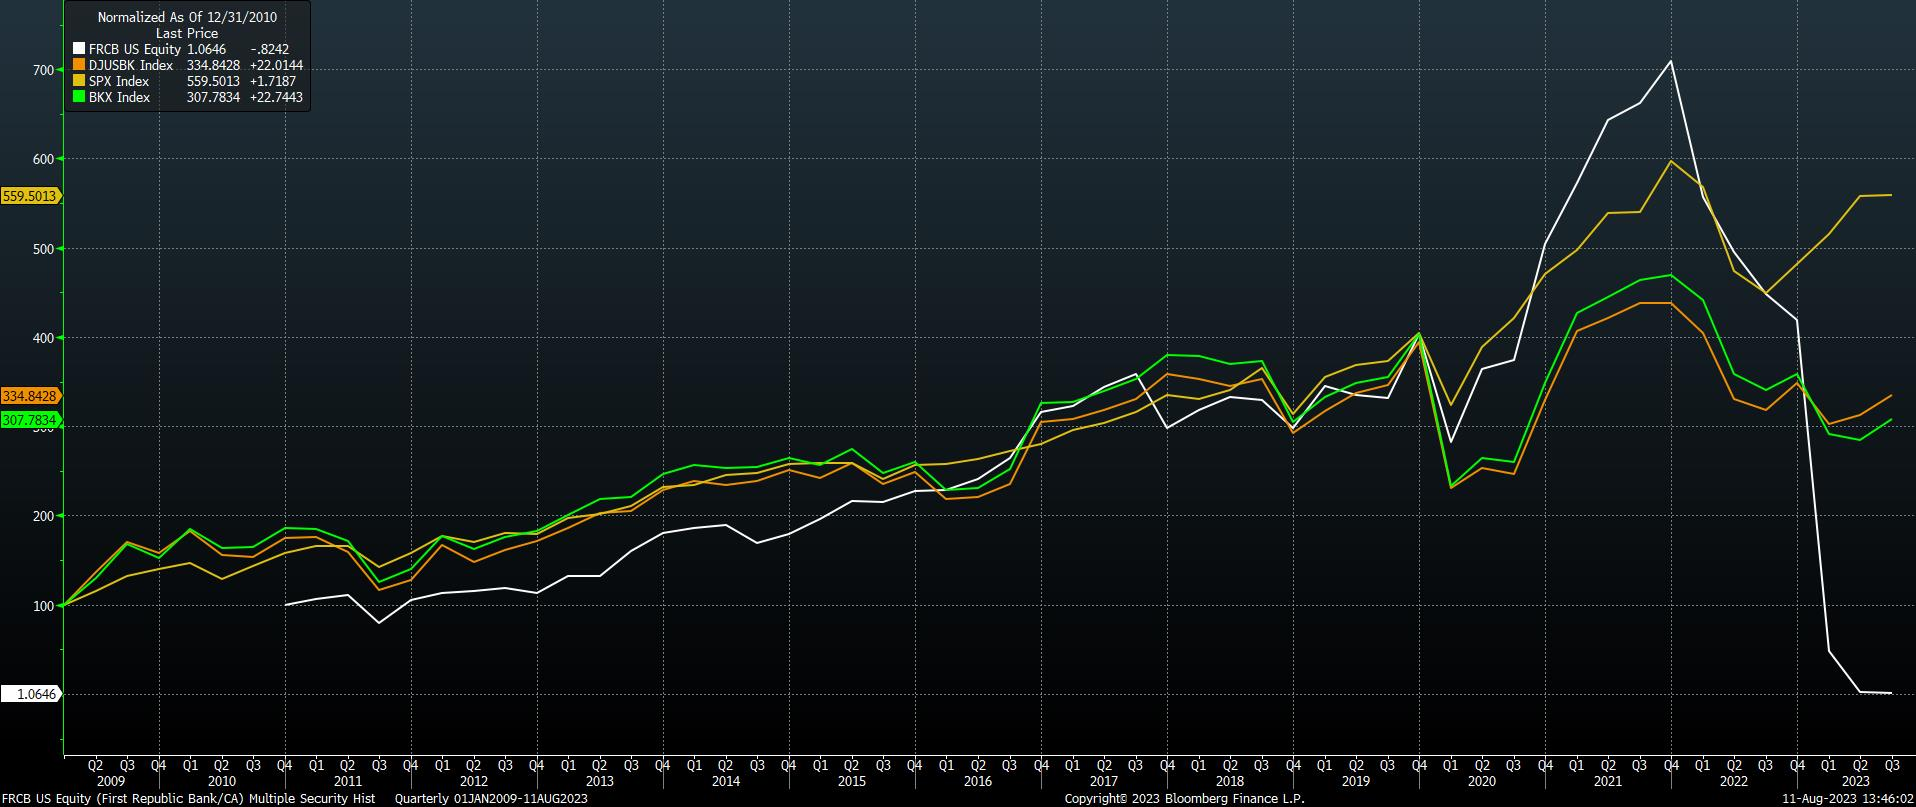
\includegraphics[scale=0.317]{images/FRCB_indexes.jpg}
    \caption{White, Brown, Kachi, and Green represent First Republic, Dow Jones U.S. Banks Index, S\&P 500 Index, and KBW NASDAQ Bank Index's prices respectively. The graph is standardized, and composed using Bloomberg.}
    \label{fig:FRC_Stock_Overall}
\end{figure}
\vspace{-0.5cm}

\subsection{The Crisis}
%-----------------------------------------The Crisis ------------------------------------
\label{The Crisis}
\vspace{-0.25cm}

\begin{itemize}
    \item On March 8th, 2023, Silicon Valley Financial Group announced they would undertake a \$2.25 billion  share sale after selling \$21 billion of securities from its portfolio at a nearly \$2 billion loss. In the next two days, the market feared the First Republic will suffer the same exposure, and investors started to sell the shares of First Republic. 
    \item On March 10th, DFPI citing inadequate liquidity and insolvency pointed to FDIC as the receiver of SVB's assets. With investors and consumers both losing the value of equity and deposits in Silicon Valley Bank, the banking sector is in a panic. Wealthy individuals and venture capitalists who have deposits above FDIC deposits insurance \$250,000 limit start withdrawing funds from the First Republic. 
    \item March 16th, 11 American banks injected the First Republic with a total of \$30 billion in uninsured deposits aimed to calm the investors and panicking consumers. However, S\&P downgraded the First Republic to junk, lowering its rating to BB+ from A-. Moody’s followed suit on Friday in cutting the bank below investment grade.
    \item March 19th, the Swiss government forced the merger of UBS and Credit Suisse for a bid of \$3.3 billion to avert a greater crisis. S\&P said it lowered First Republic’s long-term issuer credit rating to B+ from BB+. 
    \item March 24th, First Republic delivered a 41\% of deposits outflow during the first quarter of 2023 in the earnings report. Consumers and Investors completely lost faith in the First Republic, the earning report became the death certificate of the First Republic Bank. The next day, First Republic's share plumbed nearly 50\% compared to the previous day's opening, from \$16 to \$8 per share, nearly 95\% below its early March price per share.\footnote{Refer to Figure 2: Price history of SIVB, FRCB, SBNY, Dow Jones U.S. Banks Index, and KBW NASDAQ Bank Index.}
    \item On May 1st, 2023, First Republic is taken over by FDIC to become the third bank to go under followed by Signature Bank and Silicon Valley Bank. All of its assets and deposits are sold to J.P. Morgan Chase in a government auction. 
    
\end{itemize}
\newpage 

\begin{figure}
    \centering
    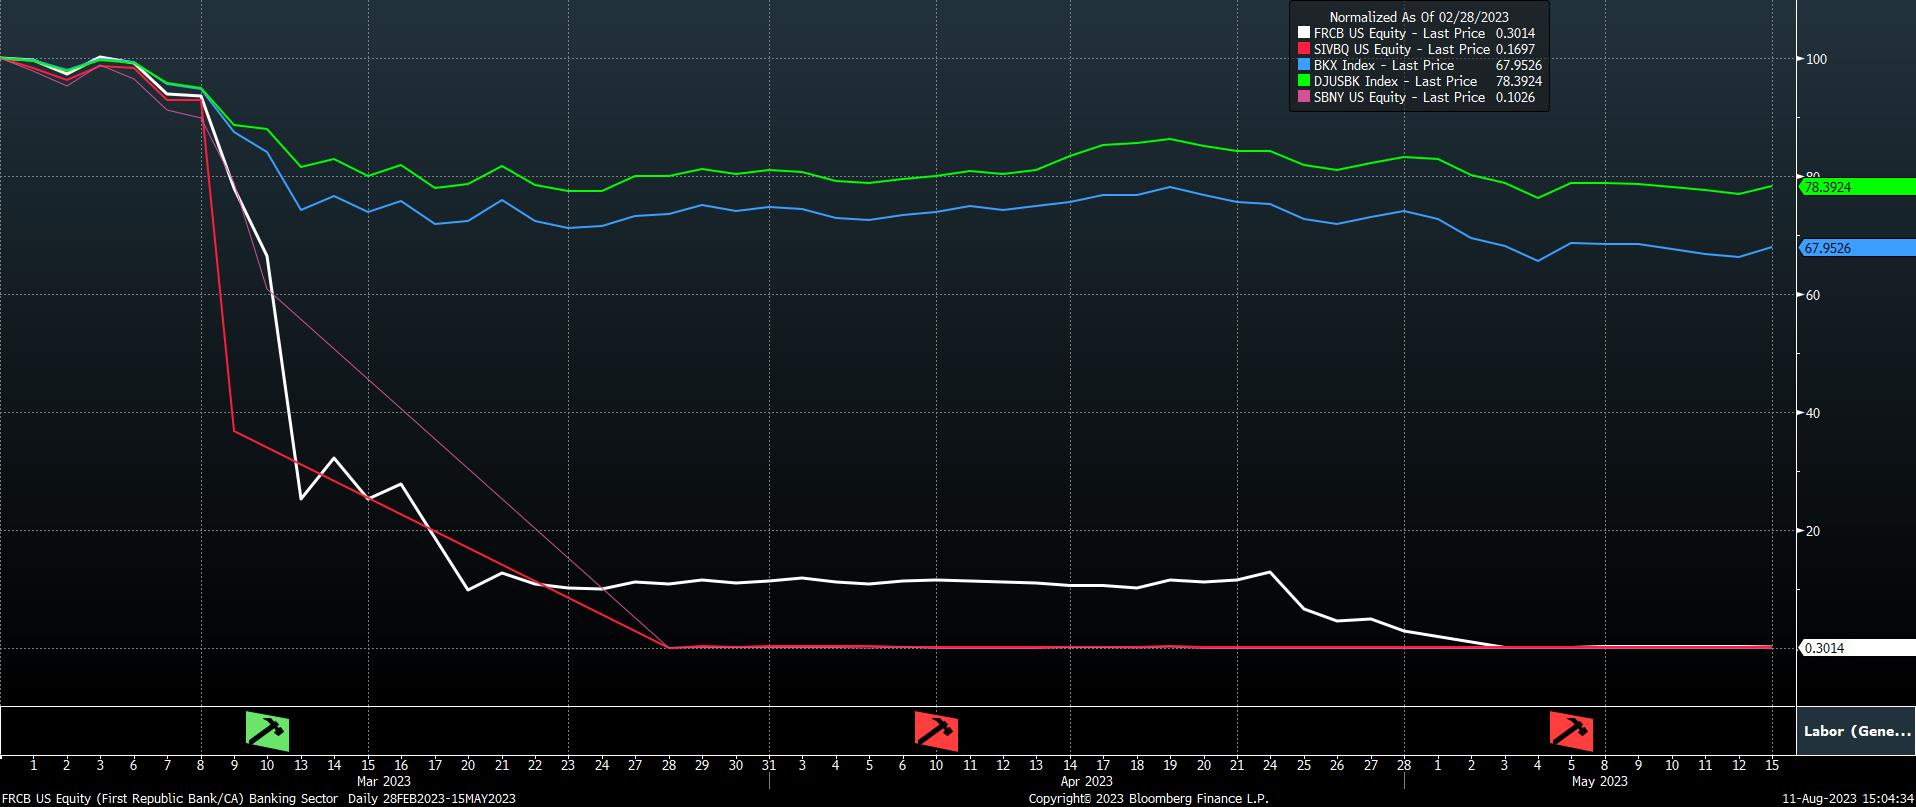
\includegraphics[scale=0.317]{images/crisis_march_may_2023.jpg}
    \caption{Price history of SIVB, FRCB, SBNY, Dow Jones U.S. Banks Index, and KBW NASDAQ Bank Index between March 1st 2023 and May 15th 2023.}
    \label{fig:enter-label}
\end{figure}


%-----------------------------------------Methodology------------------------------------
\section{Methodology - Diamond-Dybvig model} \label{Methodology}
\vspace{-0.25cm}
%-----------------------------------------Introduction to Diamond-Dybvig model ------------------------------------
\subsection{Introduction to Diamond-Dybvig model}\label{Diamond-Dybvig model}
\vspace{-0.25cm}

\quad \quad In the Diamond-Dybvig model, with the assumption of a simple economy with three time periods, as shown in \textbf{Table 1}., the banks can improve the risk sharing of simple competitive markets by transforming illiquid assets, it's shown that such banks are always vulnerable to runs. 
 Consumers will sign their insurance contract(pure demand deposit) with a financial institution - preferably a bank, to guarantee their future liquidity. Consumers will consume randomly between $\textrm{T} = 1$ and $\textrm{T} = 2$, they need the liquidity of their deposits, hence they will withdraw their deposits between the two periods. Consumers' unique financial circumstances may cause their type won't be observed until $\textrm{T} = 1$, or their choices by maximizing the utility of consumption between two periods, either way, there should be a proportion of consumers - $\theta$, who will withdraw their deposit at $\textrm{T} = 1$ and the remaining consumers - $1 - \theta$ who will withdraw at $\textrm{T} = 2$. 

If consumers withdraw at $\textrm{T} = 1$ they can only salvage their initial investment, and if consumers withdraw at $\textrm{T} = 2$ their financial investment will have a return of $\textrm{R}$, which $\textrm{R} > 1$(larger than their initial deposits). In summer in a simple economy, consumer behavior when they sign a pure demand deposits contract can be summarized in the table above. However, if the consumer types were publicly observable as of period $\textrm{T} = 1$, then the optimal consumption level satisfies $c^{1\ast}_{1} > 1$ and $c^{2\ast}_{2} < R$. (Let $c^{i}_{k} \textrm{be consumption in period } k \textrm{ of a consumer who is of type } i$).\footnote{Detailed proof refer to footnote 3 of "Bank Runs, Deposit Insurance, and Liquidity", written by Douglas W. Diamond and Philip H. Dybvig}. Under the pure demand deposit contract, the bank has to offer a fixed payment of $r_{1}$, in which $r_{1} = c^{1\ast}_{1} > 1$ for each consumer withdraw in period $\textrm{T} = 1$. Only when the fixed payment per dollar of deposits withdrawn at the period $\textrm{T} = 1$ equals the optimal consumption of Type 1 consumer, then we will have a pure strategy equilibrium for Type 1 consumer to withdraw at period $\textrm{T} = 1$ and Type 2 consumers to withdraw ta period $\textrm{T} = 2$.

However, this pure demand deposit contract has another pure strategy equilibrium, that is when all consumer panic and try to withdraw their deposits at the period $\textrm{T} = 1$, regardless of the types of consumer, all of them will try to withdraw at the period $\textrm{T} = 1$. However, besides their contracted deposits, consumers also expect their fixed payment of $r_{1}$, which is higher than their initial deposits. Bank will have to process withdrawals in sequential order by liquidating all of its assets. Even if the bank success liquidates all of its assets without any losses, it still couldn't payback all the promised fixed payments of $r_{1}$ since the higher return at the period $\textrm{T} = 1$ comes from allowing consumers to smooth consumption across both types. This is the bank-run equilibrium. 

\begin{table}[]
    \centering
    \begin{tabular}{|p{3cm}||p{3cm}||p{3cm}|p{3cm}|}
        \hline
        \textrm{Consumer Type}& \textrm{Return at T = 0}& \textrm{Return at T = 1}& \textrm{Return at T = 2}\\
        \hline
        Inpatient Consumer & -1 & 1 & 0\\
        Patient Consumer & -1 & 0 & R, (R > 1)\\
        \hline   
    \end{tabular}
    \caption{All consumers are identical as of period 0. Each faces a privately observed, uninsurable risk of being type 1 or of type 2. In period 1, each agent (consumer) learns his type.}
    \label{tab:my_label}
\end{table}

%-----------------------------------------First Republic's Financial------------------------------------
\subsection{First Republic's Financial and Bank Run equilibrium}\label{FRC Financial}
\vspace{-0.25cm}

\quad \quad From \textbf{Table 2} we are looking at the financial data from 2022:Q4 and 2023:Q1 reported by First Republic \footnote{https://news.firstrepublic.com/static-files/013f57fb-b980-4353-bbb3-0e7a3b27f20a}. Noticeably, we can see a substantially higher share of security holdings and uninsured deposits back in 2022:Q4. CET1 levels are genuinely around the same as the weighted average of all U.S. bank holding companies. The high loan concentration risk combined with the similarity among their clients that the First Republic Bank shared with the Silicon Valley Bank, the industry exposure along brings outflow of deposits the moment Silicon Valley Bank announced their mismanaged liquidity risk. 

Evidently, the First Republic still has a larger percentage of uninsured deposits than the weighted average of U.S. banks and their interest-bearing securities are taking heavy losses during the fiscal year of 2022. Every risk that Silicon Valley has been exposed to, the First Republic has experienced in their financial only on a smaller scale. Compare to Silicon Valley Bank and Signature Bank their smaller exposure to risk does buy them some time for a \$30 billion uninsured deposit injection by other largest U.S. banks on March 16th, however, because of the similarities of liquidity risk these three banks share, it surprises none when the consumers still choose bank-run equilibrium for the First Republic Bank.

From FRB Earning Release Q1 2023 as of March 31st, 2023 estimated uninsured deposits as a percentage of total deposits are 48\%, including the \$30 billion uninsured deposit injection, excluding the uninsured deposit injection, the percentage comes down to 27\%. Compare to the December 31st, 2022 data of estimated uninsured deposits as a percentage of total deposits 67\%, without accounting for government uninsured deposits injection, this is a 40\% decline of uninsured deposits solely because of deposits outflow caused by the consumers choosing bank-run equilibrium. Combine this data with a total deposit decline \$72.0 billion during a single quarter, if back on March 8th, the Silicon Valley Bank announced their liquidity issues were the matches, on April 24th the Q1 earning release of First Republic is the house filled with gasoline with turned stove on. And the next thing we know entire houses are on fire, while the consumers scramble to withdraw their deposits to avoid being on the short end of the bank-run equilibrium. 

\begin{table}[]
    \centering
    \begin{tabular}{|p{7.5cm}||p{1cm}||p{1cm}||p{2.5cm}|}
        \hline
        \textrm{Metric(Percentage)}& \textrm{2022:Q4}& \textrm{2023:Q1}& \textrm{LBOs(2022:Q4)}\\
        \hline
        Loan as a percentage of total assets & 78 & 74 & 58\\
        \hline
        Securities as a percentage of total assets & 15 & 15 & 25 \\
        \hline
        Held-to-maturity securities as a percentage of total assets & 89 & 91 & 42\\
        \hline
        Total deposits as a percentage of total liabilities & 83 & 45 & 82\\
        \hline
        Uninsured deposits as a percentage of total deposits & 67 & 48 & 41\\
        \hline
        Common equity tier 1 capital as a percentage of total risk-weighted assets & 9 & 9 & 10\\
        \hline   
    \end{tabular}
    \caption{A peer comparison, and two-quarters of self-comparison between First Republic}
    
    \label{tab:my_label}
\end{table}

%-----------------------------------------Comparioson------------------------------------
\section{Comparioson - Sillicon Valley Bank} \label{Comparioson}
\vspace{-0.25cm}

\quad \quad Among the three U.S. banks that failed in 2023, First Republic Bank manage to survive around 60 days longer, before being officially taken over by the FDIC and their assets being sold to J.P. Morgan. Observed from \textbf{Table 3}, First Republic's exposure is much more similar to Silicon Valley Bank resulting in consumers instantaneously choosing bank-run equilibrium, however, First Republic was less reckless in taking in uninsured deposits, and the percentage of uninsured deposits of total deposits are much smaller as well as less CET1 level of risk  than Silicon Valley Bank. Obviously, the main reason behind their 60-day window-of-hope is the \$30 billion uninsured deposits backed by the other largest American Banks. Despite the deposit injection by the government to ease consumer panic and increase market confidence, the rate of deterioration of First Republic's finances couldn't help but fuel their failure as they revealed a more than 40\% deposit outflow in a single quarter.

\begin{table}[]
    \centering
    \begin{tabular}{|p{7.5cm}||p{1cm}||p{1cm}||p{2.5cm}|}
        \hline
        \textrm{Metric(Percentage)}& \textrm{FRCB}& \textrm{SVBFG}\\
        \hline
        Loan as a percentage of total assets & 78 & 35\\
        \hline
        Securities as a percentage of total assets & 15 &  55 \\
        \hline
        Held-to-maturity securities as a percentage of total assets & 89 & 78\\
        \hline
        Total deposits as a percentage of total liabilities & 83 & 89\\
        \hline
        Uninsured deposits as a percentage of total deposits & 67 & 94 \\
        \hline
        Common equity tier 1 capital as a percentage of total risk-weighted assets & 9 & 12\\
        \hline   
    \end{tabular}
    \caption{A direct comparison of 2022:Q4 financial data between First Republic Bank and Silicon Valley Financial Group}
    
    \label{tab:my_label}
\end{table}

%-----------------------------------------Conclusion-----------------------------------
\section{Conclusion} \label{Conclusion}

\quad \quad As of today, the First Republic Bank's stock can only trade in OTC under the ticket name "FRCB" for 30 cents a share, all of their assets have been sold to J.P. Morgan, with that, all of their liabilities have been transferred as well. Once an industry giant at its peak having more than \$213 billion in assets now only have a market capital of 56 million. When the economy recovers from an economic recession because of the COVID pandemic with the help of government stimulus, nearly the entire banking sector are recovering fast, however, this inflow of capital incentives mismanagement of liquidity risk, and the banks let greed take over. As we can observe from \textbf{Figure 3}, in the March of 2022, Federal Reserve started to consistently increase interest rates aimed to battle inflation, then the entire banking sector quickly deflated due to the high percentage of yield-to-maturity securities holdings and the high percentage of interest-rate bearing deposits that the banks are exposed to. In the span of a year, the market's fear of banks going under became a self-full-filled prophecy and it didn't stop until 4 major bank run incidents occur back-to-back within a month to reshuffle the entire sector and tighten the government regulator's standard once again since 2008. 


\begin{figure}
    \centering
    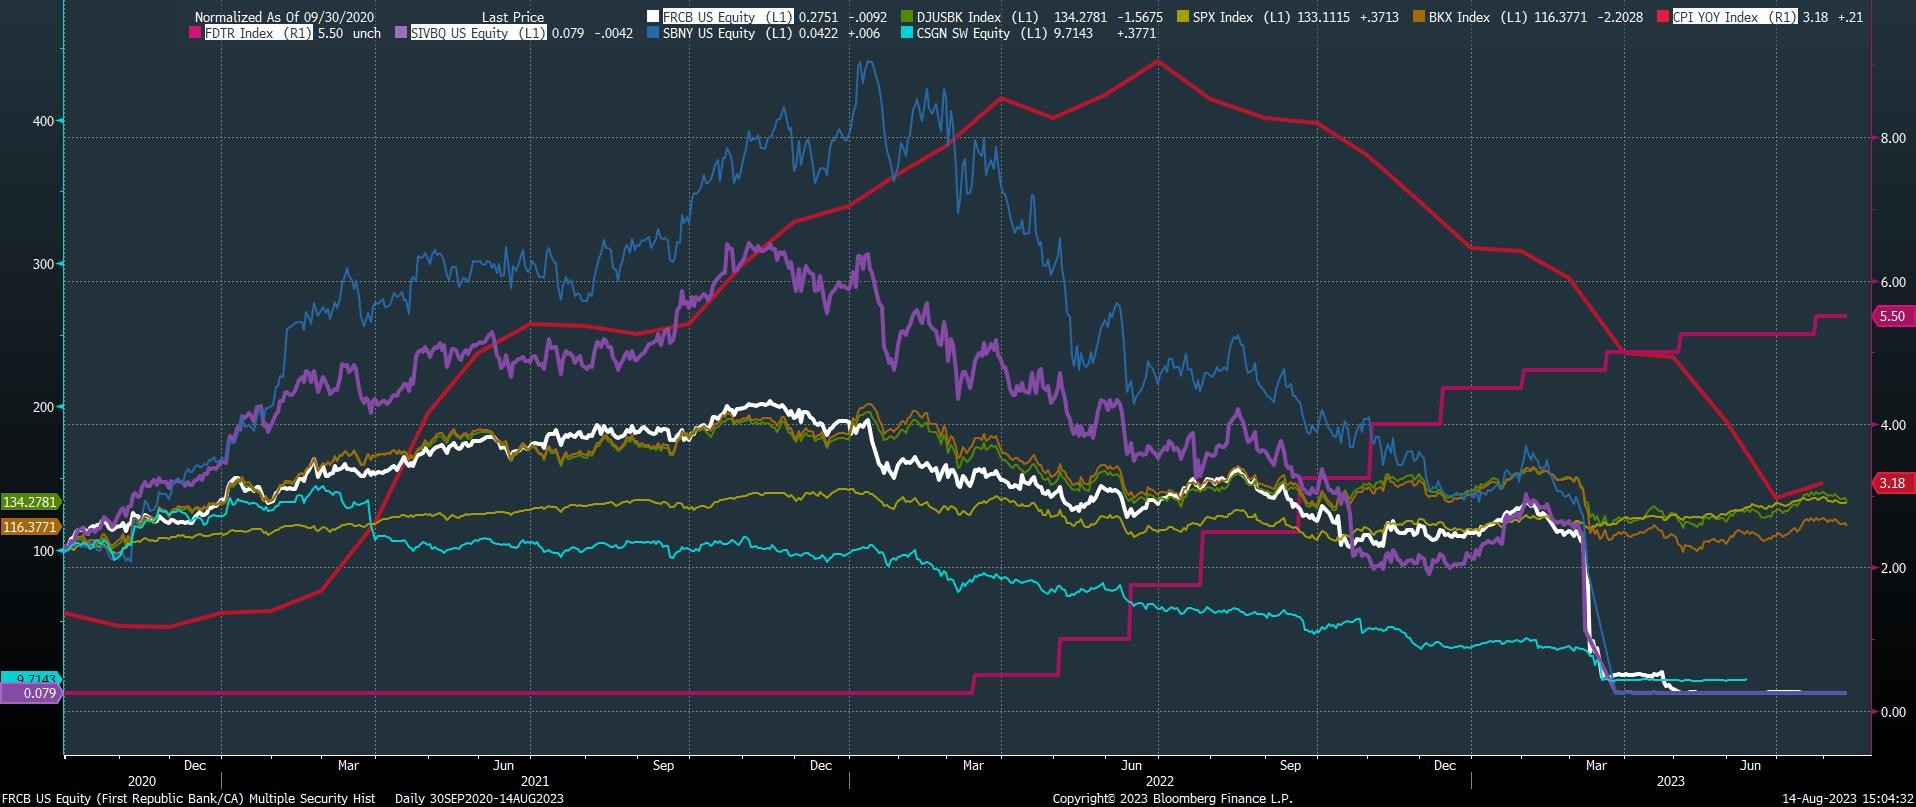
\includegraphics[scale=0.32]{images/bank_prices_cpi_fedfunds_2020_2023.jpg}
    \caption{Price history of SIVB, FRCB, SBNY, CSGN, Dow Jones U.S. Banks Index, and KBW NASDAQ Bank Index. Alongside with U.S. CPI Index and Federal Fund Target Rate between August 2020 and August 2023.}
    \label{fig:enter-label}
\end{figure}

\newpage

All in all, Silicon Valley Bank, Signature Bank, and First Republic's poor decision of mismatching liquidity with the unprecedented unrealized losses in interest-rate bearing securities and a high percentage of concentrated clients with uninsured deposits resulted in an overall stressed Banking-Sector. A heightened social media coordination and technology-enabled immediate withdraws of funding contributed to the bank runs of the third(Silicon Valley Bank) and fourth(Signature Bank) largest banks in the U.S. The high stress of the U.S. banking sector continues to pressure the First Republic resulting in more than 40\% deposits decline in a total of \$72 billion - including the \$30 billion uninsured deposit injection, in a single fiscal quarter. Even with \$30 billion of uninsured deposits injection backed up by other largest banks in the U.S., the consumers went into a complete frenzy after realizing the percentage of the withdrawal meant a majority of consumers already have chosen the bank-run equilibrium and successfully withdrawn their deposits. To avoid getting zero utility because of the sequential withdrawal order of the bank-run equilibrium, and it's inevitable at this point, even more, consumers pile in to choose bank-run equilibrium to maximize their consumption, ending the 38-year run of the 14th largest lender in the US, leaving First Republic Bank becoming the second largest bank failure in U.S. history. 

\newpage

%-----------------------------------------References-----------------------------------
\section{References} \label{References}
\begin{itemize}
    \item BOARD OF GOVERNORS OF THE FEDERAL RESERVE SYSTEM. Financial Stability Report. May 2023.

    \item Diamond, Douglas W., and Philip H. Dybvig. “Bank Runs, Deposit Insurance, and Liquidity.” Journal of Political Economy, vol. 91, no. 3, 1983.

    \item First Republic Bank. FIRST REPUBLIC REPORTS FIRST QUARTER 2023 RESULTS. 2023.

    \item Prentice, Chris, et al. “PNC, JPMorgan putting in final bids for First Republic Bank in FDIC auction.” Reuters, 2023, https://www.reuters.com/business/finance/pnc-jpm-putting-final-bids-first-republic-fdic-auction-sources-2023-04-30/.

    \item Saul, Derek. “First Republic Bank Failure: A Timeline Of What Led To The Second-Largest Bank Collapse In U.S. History.” Forbes, 2023, https://www.forbes.com/sites/dereksaul/2023/05/01/first-republic-bank-failure-a-timeline-of-what-led-to-the-second-largest-bank-collapse-in-us-history/?sh=df55c4c67b76.
    \item Tan, Gillian, and Ed Hammond. “First Republic to Face Second S\&P Downgrade in Less Than a Week.” Bloomberg News, 2023, https://www.bnnbloomberg.ca/first-republic-to-face-second-s-p-downgrade-in-less-than-a-week-1.1897626.
\end{itemize}

\newpage



\end{document}
